% Generated 2020-08-21 17:36:02 +0530
\subsection{DataItems} \label{sec:DataItems}


\block{DataItems} \glspl{organize} \block{DataItem} elements.

\begin{figure}[ht]
  \centering
    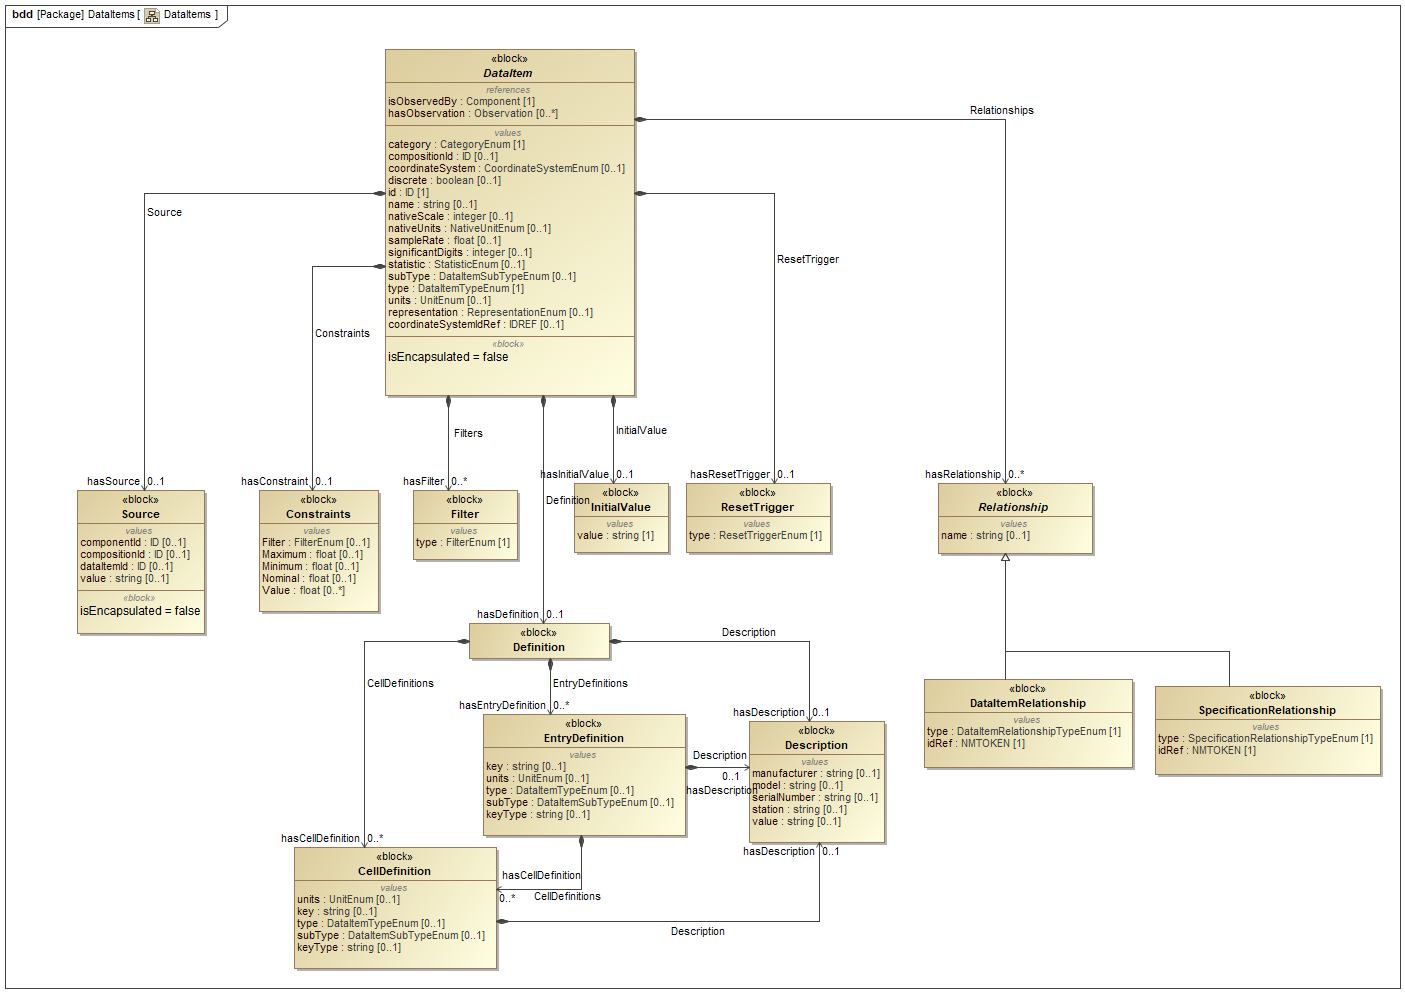
\includegraphics[width=1.0\textwidth]{figures/DataItems.png}
  \caption{DataItems Diagram}
  \label{fig:DataItems}
\end{figure}

\FloatBarrier



\subsubsection{DataItem}
\label{sec:DataItem}



\block{DataItem} describes a piece of information reported about a piece of equipment.


\paragraph{Attributes of DataItem}\mbox{}
\label{sec:Attributes of DataItem}

\tbl{Attributes of DataItem} lists the attributes of \texttt{DataItem}.

\begin{table}[ht]
\centering 
  \caption{Attributes of DataItem}
  \label{table:Attributes of DataItem}
\tabulinesep=3pt
\begin{tabu} to 6in {|l|l|l|} \everyrow{\hline}
\hline
\rowfont\bfseries {Attribute} & {Type} & {Multiplicity} \\
\tabucline[1.5pt]{}
\property{category}[DataItem] & \texttt{CategoryEnum} & 1 \\
\property{compositionId}[DataItem] & \texttt{ID} & 0..1 \\
\property{coordinateSystem}[DataItem] & \texttt{CoordinateSystemEnum} & 0..1 \\
\property{discrete}[DataItem] & \texttt{boolean} & 0..1 \\
\property{id}[DataItem] & \texttt{ID} & 1 \\
\property{name}[DataItem] & \texttt{string} & 0..1 \\
\property{nativeScale}[DataItem] & \texttt{integer} & 0..1 \\
\property{nativeUnits}[DataItem] & \texttt{NativeUnitEnum} & 0..1 \\
\property{sampleRate}[DataItem] & \texttt{float} & 0..1 \\
\property{significantDigits}[DataItem] & \texttt{integer} & 0..1 \\
\property{statistic}[DataItem] & \texttt{StatisticEnum} & 0..1 \\
\property{subType}[DataItem] & \texttt{DataItemSubTypeEnum} & 0..1 \\
\property{type}[DataItem] & \texttt{DataItemTypeEnum} & 1 \\
\property{units}[DataItem] & \texttt{UnitEnum} & 0..1 \\
\property{representation}[DataItem] & \texttt{RepresentationEnum} & 0..1 \\
\property{coordinateSystemIdRef}[DataItem] & \texttt{IDREF} & 0..1 \\
\end{tabu}
\end{table}
\FloatBarrier


Descriptions for attributes of \block{DataItem}:

\begin{itemize}
\item \property{category}[DataItem] : Specifies the kind of information provided by a data item.

\tabulinesep = 5pt
\begin{longtabu} to \textwidth {
    |l|X|}
  \caption{CategoryEnum Enumeration}
  \label{enum:CategoryEnum} \\

\hline
Name & Description \\
\hline
\endfirsthead
\hline
\multicolumn{2}{|c|}{Continuation of Table \texttt{CategoryEnum} Enumeration} \\
\hline
Name & Description \\
\hline
\endhead
\texttt{SAMPLE} & A \texttt{SAMPLE} is the reading of the value of a continuously variable or analog data value. A continuous value can be measured at any point-in-time and will always produce a result. \\ \hline
\texttt{EVENT} & An \texttt{EVENT} is a data item representing a discrete piece of information from the piece of equipment. \\ \hline
\texttt{CONDITION} & A \texttt{CONDITION} is a data item that communicates information about the health of a piece of equipment and its ability to function. \\ \hline
\end{longtabu}

\FloatBarrier
\item \property{compositionId}[DataItem] : The identifier attribute of the \block{Composition} element that the reported data is most closely associated.
\item \property{coordinateSystem}[DataItem] : For measured values relative to a coordinate system like \block{POSITION}, the coordinate system being used may be reported.

\tabulinesep = 5pt
\begin{longtabu} to \textwidth {
    |l|X|}
  \caption{CoordinateSystemEnum Enumeration}
  \label{enum:CoordinateSystemEnum} \\

\hline
Name & Description \\
\hline
\endfirsthead
\hline
\multicolumn{2}{|c|}{Continuation of Table \texttt{CoordinateSystemEnum} Enumeration} \\
\hline
Name & Description \\
\hline
\endhead
\texttt{MACHINE} & An unchangeable coordinate system that has machine zero as its origin. \\ \hline
\texttt{WORK} & The coordinate system that represents the working area for a particular workpiece whose origin is shifted within the \texttt{MACHINE} coordinate system. If the \texttt{WORK} coordinates are not currently defined in the piece of equipment, the \texttt{MACHINE}
coordinates will be used. \\ \hline
\end{longtabu}

\FloatBarrier
\item \property{discrete}[DataItem] : An indication signifying whether each value reported for the \gls{Data Entity} is significant and whether duplicate values are to be suppressed.

If a value is not defined for \property{discrete}, the default value \textbf{MUST} be \texttt{false}.
\item \property{id}[DataItem] : The unique identifier for this element.
\item \property{name}[DataItem] : The name of an element or a piece of equipment.
\item \property{nativeScale}[DataItem] : \block{nativeScale} \textbf{MAY} be used to convert the reported value to represent the original measured value.
\item \property{nativeUnits}[DataItem] : The native units of measurement for the reported value of the data item.

\tabulinesep = 5pt
\begin{longtabu} to \textwidth {
    |l|X|}
  \caption{NativeUnitEnum Enumeration}
  \label{enum:NativeUnitEnum} \\

\hline
Name & Description \\
\hline
\endfirsthead
\hline
\multicolumn{2}{|c|}{Continuation of Table \texttt{NativeUnitEnum} Enumeration} \\
\hline
Name & Description \\
\hline
\endhead
\texttt{CENTIPOISE} & A measure of viscosity. \\ \hline
\texttt{DEGREE/MINUTE} & Rotational velocity in degrees per minute. \\ \hline
\texttt{FAHRENHEIT} & Temperature in Fahrenheit. \\ \hline
\texttt{FOOT} & Feet. \\ \hline
\texttt{FOOT/MINUTE} & Feet per minute. \\ \hline
\texttt{FOOT/SECOND} & Feet per second. \\ \hline
\texttt{FOOT/SECOND\^{}2} & Acceleration in feet per second squared. \\ \hline
\texttt{FOOT\textunderscore 3D} & A point in space identified by X, Y, and Z positions and represented by a space-delimited set of numbers each expressed in feet. \\ \hline
\texttt{GALLON/MINUTE} & Gallons per minute. \\ \hline
\texttt{HOUR} & A measurement of time in hours. \\ \hline
\texttt{INCH} & Inches. \\ \hline
\texttt{INCH/MINUTE} & Inches per minute. \\ \hline
\texttt{INCH/SECOND} & Inches per second. \\ \hline
\texttt{INCH/SECOND\^{}2} & Acceleration in inches per second squared. \\ \hline
\texttt{INCH\textunderscore POUND} & A measure of torque in inch pounds. \\ \hline
\texttt{INCH\textunderscore 3D} & A point in space identified by X, Y, and Z positions and represented by a space-delimited set of numbers each expressed in inches. \\ \hline
\texttt{KELVIN} & A measurement of temperature. \\ \hline
\texttt{KILOWATT} & A measurement in kilowatt. \\ \hline
\texttt{KILOWATT\textunderscore HOUR} & Kilowatt hours which is 3.6 mega joules. \\ \hline
\texttt{LITER} & Measurement of volume of a fluid. \\ \hline
\texttt{LITER/MINUTE} & Measurement of rate of flow of a fluid. \\ \hline
\texttt{MILLIMETER/MINUTE} & Velocity in millimeters per minute. \\ \hline
\texttt{MINUTE} & A measurement of time in minutes. \\ \hline
\texttt{OTHER} & Unsupported units. \\ \hline
\texttt{POUND} & US pounds. \\ \hline
\texttt{POUND/INCH\^{}2} & Pressure in pounds per square inch (PSI). \\ \hline
\texttt{RADIAN} & Angle in radians. \\ \hline
\texttt{RADIAN/MINUTE} & Velocity in radians per minute. \\ \hline
\texttt{RADIAN/SECOND} & Rotational acceleration in radian per second squared. \\ \hline
\texttt{RADIAN/SECOND\^{}2} & Rotational acceleration in radian per second squared. \\ \hline
\texttt{REVOLUTION/SECOND} & Rotational velocity in revolution per second. \\ \hline
\end{longtabu}

\FloatBarrier
\item \property{sampleRate}[DataItem] : The rate at which successive samples of a data item are recorded by a piece of equipment.
\item \property{significantDigits}[DataItem] : The number of significant digits in the reported value.
\item \property{statistic}[DataItem] : Describes the type of statistical calculation performed on a series of data samples to provide the reported data value.

\tabulinesep = 5pt
\begin{longtabu} to \textwidth {
    |l|X|}
  \caption{StatisticEnum Enumeration}
  \label{enum:StatisticEnum} \\

\hline
Name & Description \\
\hline
\endfirsthead
\hline
\multicolumn{2}{|c|}{Continuation of Table \texttt{StatisticEnum} Enumeration} \\
\hline
Name & Description \\
\hline
\endhead
\texttt{AVERAGE} & Mathematical Average value calculated for the data item during the calculation period. \\ \hline
\texttt{KURTOSIS} & \textbf{DEPRECATED} in \textit{Version 1.6}. \sout{A measure of the "peakedness" of a probability distribution; i.e., the shape of the distribution curve.} \\ \hline
\texttt{MAXIMUM} & Maximum or peak value recorded for the data item during the calculation period. \\ \hline
\texttt{MEDIAN} & The middle number of a series of numbers. \\ \hline
\texttt{MINIMUM} & Minimum value recorded for the data item during the calculation period. \\ \hline
\texttt{MODE} & The number in a series of numbers that occurs most often. \\ \hline
\texttt{RANGE} & Difference between the maximum and minimum value of a data item during the calculation period. Also represents Peak-to-Peak measurement in a waveform. \\ \hline
\texttt{ROOT\textunderscore MEAN\textunderscore SQUARE} & Mathematical Root Mean Square (RMS) value calculated for the data item during the calculation period. \\ \hline
\texttt{STANDARD\textunderscore DEVIATION} & Statistical Standard Deviation value calculated for the data item during the calculation period. \\ \hline
\end{longtabu}

\FloatBarrier
\item \property{subType}[DataItem] : A sub-categorization of the data item \block{type}.

\tabulinesep = 5pt
\begin{longtabu} to \textwidth {
    |l|X|}
  \caption{DataItemSubTypeEnum Enumeration}
  \label{enum:DataItemSubTypeEnum} \\

\hline
Name & Description \\
\hline
\endfirsthead
\hline
\multicolumn{2}{|c|}{Continuation of Table \texttt{DataItemSubTypeEnum} Enumeration} \\
\hline
Name & Description \\
\hline
\endhead
\texttt{ABSOLUTE} & The position of a block of program code relative to the beginning of the control program. \\ \hline
\texttt{ACTION} & An indication of the operating state of a mechanism represented by a composition type component.
 The operating state indicates whether the composition element is activated or disabled. 
 The valid data value must be active value or inactive value. \\ \hline
\texttt{ACTUAL} & The measured value of the data item type given by a sensor or encoder. \\ \hline
\texttt{ALL} & The count of all the parts produced.  If the subtype is not given, this is the default. \\ \hline
\texttt{ALTERNATING} & The measurement of alternating voltage or current.   If not specified further in statistic, defaults to RMS voltage.  \\ \hline
\texttt{A\textunderscore SCALE} & A Scale weighting factor.   This is the default weighting factor if no factor is specified \\ \hline
\texttt{AUXILIARY} & When multiple locations on a piece of bar stock are referenced as the indication for the endofbar event, the additional location(s) must be designated as auxiliary subtype indication(s) for the endofbar event.   \\ \hline
\texttt{BAD} & Indicates the count of incorrect parts produced. \\ \hline
\texttt{BRINELL} & A scale to measure the resistance to deformation of a surface. \\ \hline
\texttt{B\textunderscore SCALE} & B Scale weighting factor \\ \hline
\texttt{COMMANDED} & A value specified by the controller type component. \\ \hline
\texttt{CONSUMED} & The amount of bulk material consumed from an object or container during a manufacturing process. \\ \hline
\texttt{CONTROL} & The state of the enabling signal or control logic that enables or disables the function or operation of the structural element. \\ \hline
\texttt{C\textunderscore SCALE} & C Scale weighting factor \\ \hline
\texttt{DELAY} & A piece of equipment waiting for an event or an action to occur. \\ \hline
\texttt{DIRECT} & The measurement of DC current or voltage. \\ \hline
\texttt{DRY\textunderscore RUN} & A setting or operator selection used to execute a test mode to confirm the execution of machine functions. 
 The valid data value must be on value or off value. 
 When dryrun subtype is on value, the equipment performs all of its normal functions, except no part or product is produced.  If the equipment has a spindle, spindle operation is suspended. \\ \hline
\texttt{D\textunderscore SCALE} & D Scale weighting factor \\ \hline
\texttt{EXPIRATION} & The time and date code relating to the expiration or end of useful life for a material or other physical item. \\ \hline
\texttt{FIRST\textunderscore USE} & The time and date code relating the first use of a material or other physical item. \\ \hline
\texttt{GOOD} & Indicates the count of correct parts made. \\ \hline
\texttt{INCREMENTAL} & The position of a block of program code relative to the occurrence of the last linelabel event encountered in the control program. \\ \hline
\texttt{JOG} & The feedrate specified by a logic or motion program, by a pre-set value, or set by a switch as the feedrate for the axes.  \\ \hline
\texttt{LATERAL} & An indication of the position of a mechanism that may move in a lateral direction.   The mechanism is represented by a composition type component. 
 The position information indicates whether the composition element is positioned to the right, to the left, or is in transition.  
 The valid data value must be right value, left value, or transitioning value. \\ \hline
\texttt{LEEB} & A scale to measure the elasticity of a surface. \\ \hline
\texttt{LENGTH} & A reference to a length type tool offset variable. \\ \hline
\texttt{LINE} & The state of the power source for the structural element. \\ \hline
\texttt{LINEAR} & The direction of motion of a linear motion. \\ \hline
\texttt{LOADED} & Subparts of a piece of equipment are under load. \\ \hline
\texttt{MACHINE\textunderscore AXIS\textunderscore LOCK} & A setting or operator selection that changes the behavior of the controller on a piece of equipment. 
 The valid data value must be on value or off value. 
 When machineaxislock subtype is on value, program execution continues normally, but no equipment motion occurs  \\ \hline
\texttt{MAIN} & The identity of the primary logic or motion program currently being executed. It is the starting nest level in a call structure and may contain calls to sub programs. \\ \hline
\texttt{MAINTENANCE} & Action related to maintenance on the piece of equipment. \\ \hline
\texttt{MANUAL\textunderscore UNCLAMP} & An indication of the state of an operator controlled interlock that can inhibit the ability to initiate an unclamp action of an electronically controlled chuck.
 The valid data value must be active value or inactive value. 
 When manualunclamp subtype is active value, it is expected that a chuck cannot be unclamped until manualunclamp subtype is set to inactive value.  \\ \hline
\texttt{MANUFACTURE} & The time and date code relating to the production of a material or other physical item. \\ \hline
\texttt{MAXIMUM} & Maximum value of a data entity or attribute. \\ \hline
\texttt{MINIMUM} & The minimum value of a data entity or attribute. \\ \hline
\texttt{MOHS} & A scale to measure the resistance to scratching of a surface. \\ \hline
\texttt{MOTION} & An indication of the open or closed state of a mechanism.   The mechanism is represented by a composition type component. 
 The operating state indicates whether the state of the composition element is open, closed, or unlatched.   
 The valid data value must be open value, unlatched value, or closed value. \\ \hline
\texttt{NO\textunderscore SCALE} & No weighting factor on the frequency scale \\ \hline
\texttt{OPERATING} & A piece of equipment are powered or performing any activity. \\ \hline
\texttt{OPERATOR} & The identifier of the person currently responsible for operating the piece of equipment. \\ \hline
\texttt{OPTIONAL\textunderscore STOP} & A setting or operator selection that changes the behavior of the controller on a piece of equipment. 
 The valid data value must be on value or off value.
 The program execution is stopped after a specific program block is executed when optionalstop subtype is on value.    
 In the case of a G-Code program, a program block event containing a M01 code designates the command for an optionalstop subtype. 
 execution event must change to optionalstop subtype after a program block specifying an optional stop is executed and the optionalstop subtype selection is on value. \\ \hline
\texttt{OVERRIDE} & DEPRECATED: The operators overridden value. \\ \hline
\texttt{POWERED} & Primary  power is  applied  to the  piece  of  equipment and,  as  a minimum, the controller or logic portion of the piece of equipment is powered and functioning or components that are required to remain on are powered. \\ \hline
\texttt{PRIMARY} & Specific applications MAY reference one or more locations on a piece of bar stock as the indication for the endofbar event. The main or most important location must be designated as the primary subtype indication for the endofbar event.   
 If no subtype is specified, primary subtype must be the default endofbar event indication. \\ \hline
\texttt{PROBE} & The position provided by a measurement probe. \\ \hline
\texttt{PROCESS} & The measurement of the time from the beginning of production of a part or product on a piece of equipment until the time that production is complete for that part or product on that piece of equipment.  This includes the time that the piece of equipment is running, producing parts or products, or in the process of producing parts. \\ \hline
\texttt{PROGRAMMED} & The value of a signal or calculation specified by a logic or motion program or set by a switch. \\ \hline
\texttt{RADIAL} & A reference to a radial type tool offset variable. \\ \hline
\texttt{RAPID} & The value of a signal or calculation issued to adjust the feedrate of a component or composition that is operating in a rapid positioning mode. \\ \hline
\texttt{REMAINING} & Remaining measure of an object or an action. \\ \hline
\texttt{ROCKWELL} & A scale to measure the resistance to deformation of a surface. \\ \hline
\texttt{ROTARY} & The rotational direction of a rotary motion using the right hand rule convention.
 The valid data value must be clockwise value or counterclockwise value. \\ \hline
\texttt{SCHEDULE} & The identity of a control program that is used to specify the order of execution of other programs. \\ \hline
\texttt{SET\textunderscore UP} & The identifier of the person currently responsible for preparing a piece of equipment for production or restoring the piece of equipment to a neutral state after production. \\ \hline
\texttt{SHORE} & A scale to measure the resistance to deformation of a surface. \\ \hline
\texttt{SINGLE\textunderscore BLOCK} & A setting or operator selection that changes the behavior of the controller on a piece of equipment. 
 The valid data value must be on value or off value.
 Program execution is paused after each block event of code is executed when singleblock subtype is on value.   
 When singleblock subtype is on value, execution event must change to interrupted value after completion of each block event of code.  \\ \hline
\texttt{STANDARD} & The standard or original length of an object. \\ \hline
\texttt{START} & The time and date associated with the beginning of an activity or event. \\ \hline
\texttt{SWITCHED} & An indication of the activation state of a mechanism represented by a composition type component.
 The activation state indicates whether the composition element is activated or not.
 The valid data value must be on value or off value. \\ \hline
\texttt{TARGET} & The desired measure or count for a data item value. \\ \hline
\texttt{TARGET\textunderscore COMPLETION} & The projected time and date associated with the end or completion of an activity or event. \\ \hline
\texttt{TOOL\textunderscore CHANGE\textunderscore STOP} & A setting or operator selection that changes the behavior of the controller on a piece of equipment. 
 The valid data value must be on value or off value. 
 Program execution is paused when a command is executed requesting a cutting tool to be changed. 
 execution event must change to interrupted value after completion of the command requesting a cutting tool to be changed and toolchangestop subtype is on value. \\ \hline
\texttt{USEABLE} & The remaining useable length of an object. \\ \hline
\texttt{VERTICAL} & An indication of the position of a mechanism that may move in a vertical direction. The mechanism is represented by a composition type component. 
 The position information indicates whether the composition element is positioned to the top, to the bottom, or is in transition.  
 The valid data value must be up value, down value, or transitioning value. \\ \hline
\texttt{VICKERS} & A scale to measure the resistance to deformation of a surface. \\ \hline
\texttt{WORKING} & A piece of equipment performing any activity, the equipment is active and performing a function under load or not. \\ \hline
\texttt{IPV4\textunderscore ADDRESS} & The IPV4 network address of the component. \\ \hline
\texttt{IPV6\textunderscore ADDRESS} & The IPV6 network address of the component. \\ \hline
\texttt{GATEWAY} & The Gateway for the component network. \\ \hline
\texttt{SUBNET\textunderscore MASK} & The SubNet mask for the component network.
 \\ \hline
\texttt{VLAN\textunderscore ID} & The layer2 Virtual Local Network (VLAN) ID for the component network. \\ \hline
\texttt{MAC\textunderscore ADDRESS} & Media Access Control Address. The unique physical address of the network hardware. \\ \hline
\texttt{WIRELESS} & Identifies whether the connection type is wireless. \\ \hline
\texttt{LICENSE} & The license code to validate or activate the hardware or software. \\ \hline
\texttt{VERSION} & The version of the hardware or software.
 \\ \hline
\texttt{RELEASE\textunderscore DATE} & The date the hardware or software was released for general use. \\ \hline
\texttt{INSTALL\textunderscore DATE} & The date the hardware or software was installed. \\ \hline
\texttt{MANUFACTURER} & The corporate identity for the maker of the hardware or software \\ \hline
\end{longtabu}

\FloatBarrier
\item \property{type}[DataItem] : The type of either a \gls{Structural Element} or a \block{DataItem} being measured.

\tabulinesep = 5pt
\begin{longtabu} to \textwidth {
    |l|X|}
  \caption{DataItemTypeEnum Enumeration}
  \label{enum:DataItemTypeEnum} \\

\hline
Name & Description \\
\hline
\endfirsthead
\hline
\multicolumn{2}{|c|}{Continuation of Table \texttt{DataItemTypeEnum} Enumeration} \\
\hline
Name & Description \\
\hline
\endhead
\end{longtabu}

\FloatBarrier
\item \property{units}[DataItem] : The unit of measurement for the reported value of the data item.

\tabulinesep = 5pt
\begin{longtabu} to \textwidth {
    |l|X|}
  \caption{UnitEnum Enumeration}
  \label{enum:UnitEnum} \\

\hline
Name & Description \\
\hline
\endfirsthead
\hline
\multicolumn{2}{|c|}{Continuation of Table \texttt{UnitEnum} Enumeration} \\
\hline
Name & Description \\
\hline
\endhead
\texttt{AMPERE} & Amps \\ \hline
\texttt{CELSIUS} & Degrees Celsius \\ \hline
\texttt{COUNT} & A count of something. \\ \hline
\texttt{DECIBEL} & Sound Level \\ \hline
\texttt{DEGREE} & Angle in degrees \\ \hline
\texttt{DEGREE\textunderscore 3D} & A space-delimited, floating-point representation of the angular rotation in degrees around the X, Y, and Z axes relative to a cartesian coordinate system respectively in order as A, B, and C. If any of the rotations is not known, it \textbf{MUST} be zero (0). \\ \hline
\texttt{DEGREE/SECOND} & Angular degrees per second \\ \hline
\texttt{DEGREE/SECOND\^{}2} & Angular acceleration in degrees per second squared \\ \hline
\texttt{HERTZ} & Frequency measured in cycles per second \\ \hline
\texttt{JOULE} & A measurement of energy. \\ \hline
\texttt{KILOGRAM} & Kilograms \\ \hline
\texttt{LITER} & Measurement of volume of a fluid \\ \hline
\texttt{LITER/SECOND} & Liters per second \\ \hline
\texttt{MICRO\textunderscore RADIAN} & Measurement of Tilt \\ \hline
\texttt{MILLIMETER} & Millimeters \\ \hline
\texttt{MILLIMETER\textunderscore 3D} & A point in space identified by X, Y, and Z positions and represented by a space-delimited set of numbers each expressed in millimeters. \\ \hline
\texttt{MILLIMETER/REVOLUTION} & Millimeters per revolution. \\ \hline
\texttt{MILLIMETER/SECOND} & Millimeters per second \\ \hline
\texttt{MILLIMETER/SECOND\^{}2} & Acceleration in millimeters per second squared \\ \hline
\texttt{NEWTON} & Force in Newtons \\ \hline
\texttt{NEWTON\textunderscore METER} & Torque, a unit for force times distance. \\ \hline
\texttt{OHM} & Measure of Electrical Resistance \\ \hline
\texttt{PASCAL} & Pressure in Newtons per square meter \\ \hline
\texttt{PASCAL\textunderscore SECOND} & Measurement of Viscosity \\ \hline
\texttt{PERCENT} & Percentage \\ \hline
\texttt{PH} & A measure of the acidity or alkalinity of a solution. \\ \hline
\texttt{REVOLUTION/MINUTE} & Revolutions per minute \\ \hline
\texttt{SECOND} & A measurement of time. \\ \hline
\texttt{SIEMENS/METER} & A measurement of Electrical Conductivity \\ \hline
\texttt{VOLT} & Volts \\ \hline
\texttt{VOLT\textunderscore AMPERE} & The measurement of the apparent power in an electrical circuit, equal to the product of root-mean-square (RMS) voltage and RMS current (commonly referred to as VA). \\ \hline
\texttt{VOLT\textunderscore AMPERE\textunderscore REACTIVE} & The measurement of reactive power in an AC electrical circuit (commonly referred to as VAR). \\ \hline
\texttt{WATT} & Watts \\ \hline
\texttt{WATT\textunderscore SECOND} & Measurement of electrical energy, equal to one Joule \\ \hline
\texttt{REVOLUTION/SECOND} & Revolutions per second. \\ \hline
\texttt{REVOLUTION/SECOND\^{}2} & Revolutions per second squared. \\ \hline
\texttt{GRAM/CUBIC\textunderscore METER} & Gram per cubic meter. \\ \hline
\texttt{CUBIC\textunderscore MILLIMETER} & Geometric volume in millimeters. \\ \hline
\texttt{CUBIC\textunderscore MILLIMETER/SECOND} & Change of geometric volume per second. \\ \hline
\texttt{CUBIC\textunderscore MILLIMETER/SECOND\^{}2} & Change in geometric volume per second squared. \\ \hline
\texttt{MILLIGRAM} & Milligram. \\ \hline
\texttt{MILLIGRAM/CUBIC\textunderscore MILLIMETER} & Milligram per cubic millimeter. \\ \hline
\texttt{MILLILITER} & Milliliter. \\ \hline
\end{longtabu}

\FloatBarrier
\item \property{representation}[DataItem] : Description of a means to interpret data consisting of multiple data points or samples reported as a single value.  

If \property{representation} is not specified, it \textbf{MUST} be determined to be \texttt{VALUE}.


\tabulinesep = 5pt
\begin{longtabu} to \textwidth {
    |l|X|}
  \caption{RepresentationEnum Enumeration}
  \label{enum:RepresentationEnum} \\

\hline
Name & Description \\
\hline
\endfirsthead
\hline
\multicolumn{2}{|c|}{Continuation of Table \texttt{RepresentationEnum} Enumeration} \\
\hline
Name & Description \\
\hline
\endhead
\texttt{TIME\textunderscore SERIES} & A series of sampled data.

The data is reported for a specified number of samples and each sample is reported with a fixed period. \\ \hline
\texttt{VALUE} & The measured value of the sample data.

If no \property{representation}[DataItem] is specified for a data item, the \property{representation}[DataItem] \textbf{MUST} be determined to be \texttt{VALUE}. \\ \hline
\texttt{DATA\textunderscore SET} & The reported value(s) are represented as a set of \glspl{key-value pair}.

Each reported value in the \gls{Data Set} \textbf{MUST} have a unique key. \\ \hline
\texttt{DISCRETE} & \textbf{DEPRECATED} as a \property{representation} in \textit{MTConnect Version. 1.5}. Replaced by the \property{discrete}[DataItem] attribute of a \block{DataItem}. \\ \hline
\texttt{TABLE} & A \gls{Table} is a two dimensional set of \glspl{key-value pair} where the \block{Entry} represents a row, and the value is a set of \gls{key-value pair} \block{Cell} elements. The \gls{Table} follows the same behavior as the \gls{Data Set} for change tracking, clearing, and history. When an \block{Entry} changes, all \block{Cell} elements update as a single unit following the behavior of a \gls{Data Set}.

Note 1 to Entry: It is best to use the \block{Variable} \block{DataItem} \property{type} if the \block{Cell} elements represent multiple
semantic types.

Each \block{Entry} in the \gls{Table} \textbf{MUST} have a unique key. Each \block{Cell} of each \block{Entry} in the \gls{Table} \textbf{MUST} have a unique key.

See \textit{Section 5.6.5} of \citetitle{MTCPart3}, for a description of
\block{Entry} and \block{Cell} elements. \\ \hline
\end{longtabu}

\FloatBarrier
\item \property{coordinateSystemIdRef}[DataItem] : The associated \block{CoordinateSystem} context for the \block{DataItem}.
\end{itemize}

\paragraph{Elements of DataItem}\mbox{}
\label{sec:Elements of DataItem}

\tbl{Elements of DataItem} lists the elements of \texttt{DataItem}.

\begin{table}[ht]
\centering 
  \caption{Elements of DataItem}
  \label{table:Elements of DataItem}
\tabulinesep=3pt
\begin{tabu} to 6in {|l|l|l|} \everyrow{\hline}
\hline
\rowfont\bfseries {Element Name} & {Type} & {Multiplicity} \\
\tabucline[1.5pt]{}
\block{Source} & \texttt{Source} & 0..1 \\
\block{Constraints} & \texttt{Constraints} & 0..1 \\
\block{Filters} & \texttt{Filter} & 0..* \\
\block{InitialValue} & \texttt{InitialValue} & 0..1 \\
\block{ResetTrigger} & \texttt{ResetTrigger} & 0..1 \\
\block{Definition} & \texttt{Definition} & 0..1 \\
\end{tabu}
\end{table}
\FloatBarrier


Descriptions for elements of \block{DataItem}:

\begin{itemize}
\item \block{Source} : \block{Source} identifies the \block{Component}, \block{DataItem}, or \block{Composition} representing the area of the piece of equipment from which a measured value originates.
\item \block{Constraints} : \block{Constraints} \glspl{organize} a set of expected values that can be reported for this \block{DataItem}.
\item \block{Filters} : \block{Filters} \glspl{organize} the \block{Filter} elements associated with this \block{DataItem} element. 
\item \block{InitialValue} : \block{InitialValue} defines the starting value for a data item as well as the value to be set for the data item after a reset event.
\item \block{ResetTrigger} : \block{ResetTrigger} identifies the type of event that may cause a reset to occur.
\item \block{Definition} : The \block{Definition} defines the meaning of \block{Entry} and \block{Cell} elements associated with the \block{DataItem} when the \property{representation} is either \block{DATA} or \block{TABLE}.
\end{itemize}
\FloatBarrier
